\subsection{Project Requirement Specifications}
\noindent The table below contains constraints for 1) hardware functionality, 2) software techniques, 3) system performance metrics, and 4) physical footprint. Some of these requirements will be further defined and derived in the longer research paper. The main constraint is time, as this project needs to be completed in the 8-month period concurrent with the senior design I \& II courses. One other constraint is the use of a pre-built walker. We are not mechanically designing the walker frame itself.

\begin{figure}[H]
	\centering
	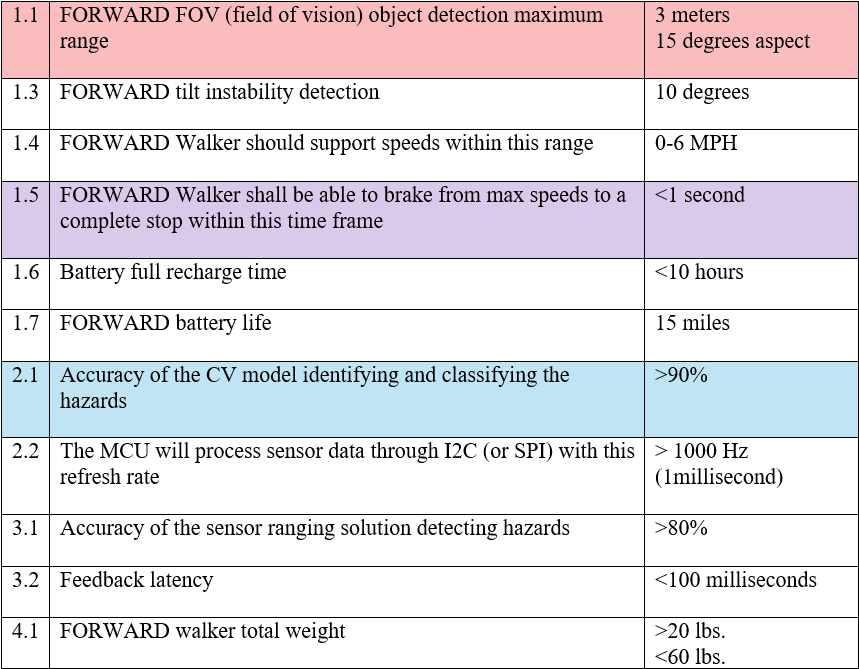
\includegraphics[width=0.99925\textwidth]{./Images/EngineeringReq.png}
	\caption{\label{fig:Standards}Engineering Requirements}
\end{figure}